%%==================================================
%% chapter03.tex for SJTU Master Thesis
%% Encoding: UTF-8
%%==================================================
% \bibliography{../bib/chap1,../bib/chap2}

\chapter{CUDA计算框架}
  CUDA是NVIDIA的GPGPU模型,它使用C语言为基础,可以直接以大多数人熟悉的C语言,写出在显示芯片上执行的程序,而不需要去学习特定的显示芯片的指令或是特殊的结构\cite{nvidia2011nvidia}。
  \par
  在CUDA的架构下,一个程序分为两个部份:host端和device端。Host端是指在CPU上执行的部份,而device端则是在显示芯片上执行的部份。Device端的程序又称为kernel。通常host端程序会将数据准备好后,复制到显卡的内存中,再由显示芯片执行device端程序,完成后再由host端程序将结果从显卡的内存中取回。
  \section{GPU与CPU的对比}
    CPU和GPU各有所长,一般而言,CPU擅长处理不规则数据结构和不可预测的存取模式,以及递归算法、分支密集型代码和单线程程序。这类程序任务拥有复杂的指令调度、循环、分支、逻辑判断以及执行等步骤。例如,操作系统、文字处理、交互性应用的除错、通用计算、系统控制和虚拟化技术等系统软件和通用应用程序等等。而GPU擅于处理规则数据结构和可预测存取模式。例如,光影处理、3D 坐标变换、油气勘探、金融分析、医疗成像、有限元、基因分析和地理信息系统以及科学计算等方面的应用。显示芯片通常具有更大的内存带宽。具有更大量的执行单元。和高阶 CPU 相比,显卡的价格较为低廉。
    \begin{figure}[htp]
      \centering
      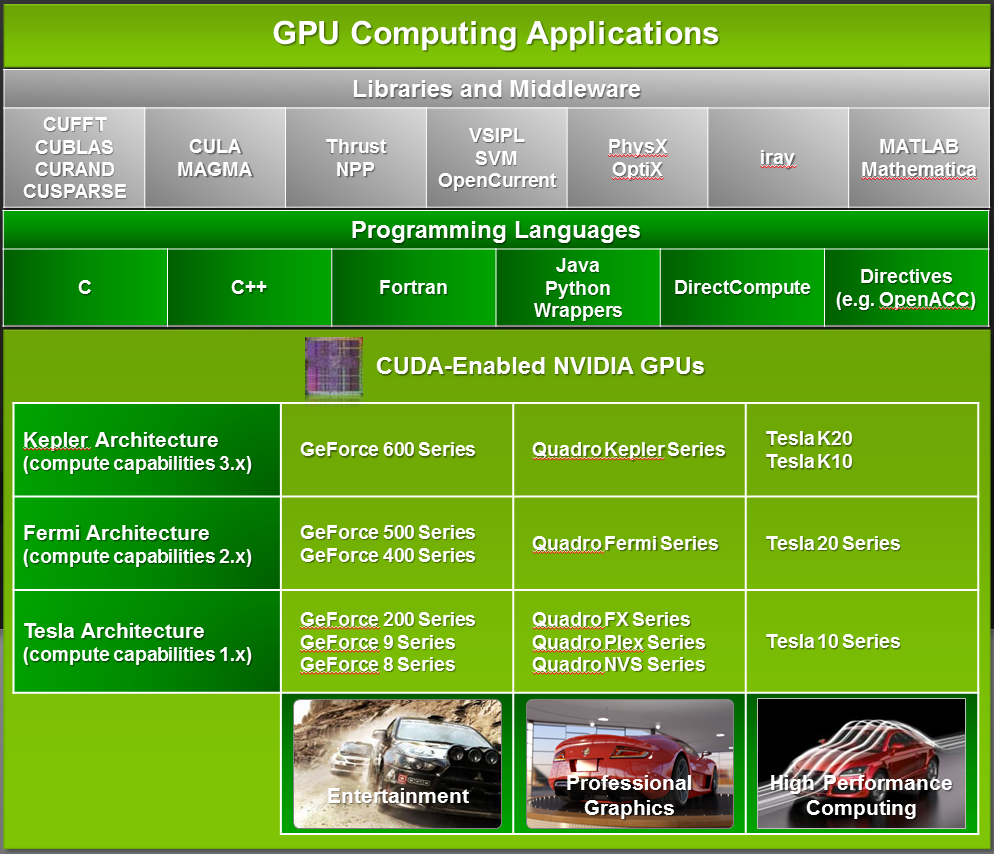
\includegraphics[width=0.7\textwidth]{chap3/application}
      \caption{GPU的应用范围}
    \end{figure}
    \par
    目前设计GPU+CPU架构平台的指导思想是:让CPU的更多资源用于缓存,GPU的更多资源用于数据计算。把两者放在一起,不但可以减小在传输带宽上的花销,还可以让CPU和GPU这两个PC中运算速度最快的部件互为帮衬。其原因是,CPU中的运算器通常只有几个ALU,而GPU中的ALU则比CPU的数目多很多。另外,CPU中高速缓存相对比较多,而GPU中的高速缓存则比CPU少很多。必要的时候,CPU可以帮助GPU分担一部分软件渲染工作,另一方面GPU可以使用主流编程语言来处理通用计算问题。这就相当于CPU多了一个强大的浮点运算部件,而GPU多了一个像素处理单元。
    \par
    从微架构上看,CPU和GPU看起来完全不是按照相同的设计思路设计的,当代CPU的微架构是按照兼顾指令并行执行和数据并行运算的思路而设计,就是要兼顾程序执行和数据运算的并行性、通用性以及它们的平衡性。CPU的微架构偏重于程序执行的效率,不会一味追求某种运算极致速度而牺牲程序执行的效率。GPU的微架构就是面向适合于矩阵类型的数值计算而设计的,大量重复设计的计算单元,这类计算可以分成众多独立的数值计算大量数值运算的线程,而且数据之间没有像程序执行的那种逻辑关联性。
    \par
    从主频上来看,GPU执行每个数值计算的速度并没有比CPU快,从目前主流CPU和GPU的主频就可以看出了,CPU的主频都超过了1GHz,2GHz,甚至3GHz,而GPU的主频最高还不到1GHz,主流的也就500~600MHz。所以GPU在执行少量线程的数值计算时并不能超过CPU。
    \par
    从每个时钟周期执行的指令数来看,这个方面,CPU和GPU无法比较,因为GPU大多数指令都是面向数值计算的,少量的控制指令也无法被操作系统和软件直接使用。如果比较数据指令的IPC,GPU显然要高过CPU,因为并行的原因。但是,如果比较控制指令的IPC,自然是CPU的要高的多。原因很简单,CPU着重的是指令执行的并行性。
    \begin{figure}[htp]
      \centering
      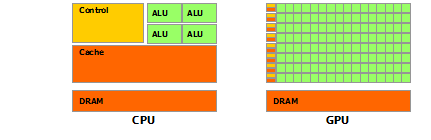
\includegraphics[width=0.7\textwidth]{chap3/gpuvscpu}
      \caption{GPU与CPU的结构区别}
    \end{figure}
    在这种架构下,GPU芯片提供了比CPU更多的计算性能与带宽。
    \begin{figure}[htp]
      \centering
      \subfigure[计算能力]{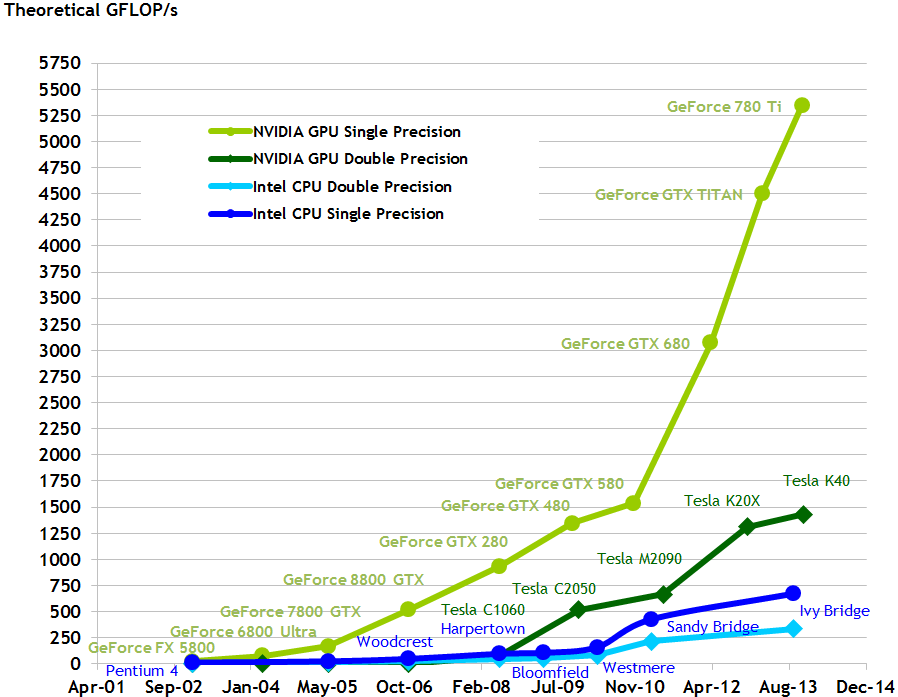
\includegraphics[width=0.4\textwidth]{chap3/compute}}
      \hspace{1cm}
      \subfigure[数据带宽]{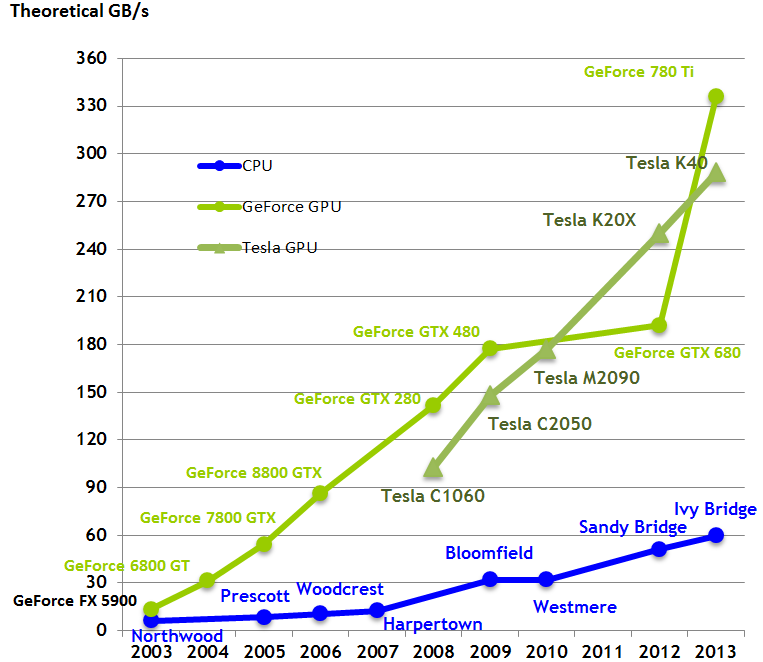
\includegraphics[width=0.4\textwidth]{chap3/bandwidth}}
      \caption{GPU与CPU性能对比}
    \end{figure}
    GPU 的设计能使更多晶体管用于数据处理,而非数据缓存和流控制。
    \par
    更具体地说,GPU 专用于解决可表示为数据并行计算的问题在许多数据元素上并行执行的程序,具有极高的计算密度(数学运算与存储器运算的比率)。由于所有数据元素都执行相同的程序,因此对精密流控制的要求不高;由于在许多数据元素上运行,且具有较高的计算密度,因而可通过计算隐藏存储器访问延迟,而不必使用较大的数据缓存。
  \section{GPU的计算模型}
    CUDA并行模型是为了降低并行开发的难度,将其应用到C等语言当中。在并行计算单中重要的三个概念:
    \begin{enumerate}
      \item 线程组的层级
      \item 共享内存
      \item 同步的范围
    \end{enumerate}
    被作为C语言的扩展暴露给开发者了。这三个功能提供细粒度的数据与线程并行\cite{cook2013cuda},以及粗粒度的数据与任务并行。这指引开发者将问题分割成可以在块与线程中独立执行的子问题,并且子问题的解决方法是类似的。这种分割防止语言过多的处理底层信息,也无需考虑不同子问题在实际运行中是并行还是串行执行,使代码与底层相互独立,无需在编写时考虑实际运行时的核心数量。为了完成这项功能,CUDA运行时可以根据流处理器的数量自动控制运行参数。
    \par
    这个模型让CUDA代码可以在不同的GPU体系结构上运行,从高性能娱乐级的GeForce系列GPU到专业级Quadro系列GPU以及高性能计算领域的Tesla系列GPU。automatic-scalability
    \begin{figure}[htp]
      \centering
      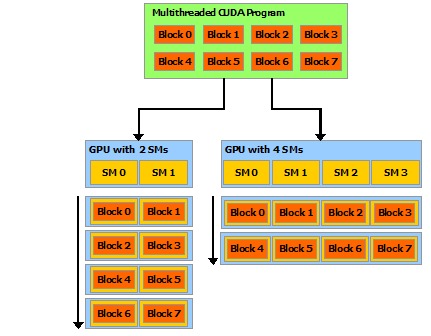
\includegraphics[width=0.5\textwidth]{chap3/automatic-scalability}
      \caption{自动控制执行}
    \end{figure}
    \subsection{核(Kernel)}
      CUDA C扩展了C语言,定义了Kernel为在GPU上运行的函数。这是由于这个核心可以被多个不同的CUDA线程执行,与只执行一次的普通C函数相对应。
      \par
      一个核函数通过\fbox{\tt \_\_global\_\_}关键字来定义,并且在执行时可以定义由多少个线程与块来执行。由于所在线程不同,每个函数在执行时都会获取一个threadIdx变量,通常情况下这个变量是一个三维的向量。
    \subsection{线程层级}
      由于CUDA可以支持三维的线程块,所以一个线程可以被一个最多三维的向量索引来决定。这提供了一个自然的索引方式来处理不同类型元素,如向量、矩阵、流量。
      \par
      线程的真实索引可以被很容易的计算出来,对于一维块,两个索引相同;对于大小为$(D_x,D_y)$的二维块,线程的真实索引$(x,y)$是$(x+yD_x)$;对于一个三维的块$(D_x,D_y,D_z)$,线程的实际索引是$(x+yD_z+zD_xD_y)$。
      \par
      由于体系结构限制,在一个块中的所有线程共享有限的共享内存与一个SM,所以,每个块中的线程数量是有限的,目前的体系结构中,每个块最多包含1024个线程。
      \par
      但是核函数也可以被多个相同的线程块执行,所以线程的总数由GPU实际的核心数限制,线程块也可以被组织为最多三维。线程块的数量可以被数据或者系统中的流处理器的量限制,但是由于不同的线程块的关联不大,线程块的数量可以比流处理器大很多。
      \begin{figure}[htp]
        \centering
        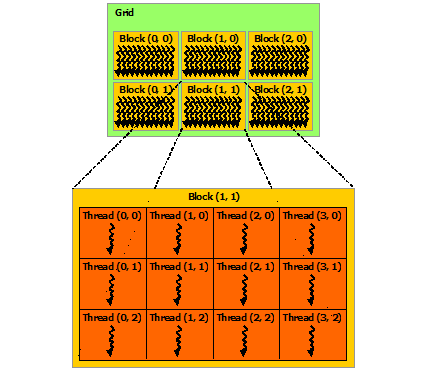
\includegraphics[width=0.5\textwidth]{chap3/grid-of-thread-blocks}
        \caption{线程、线程块与网格}
      \end{figure}
      每个线程都可以通过内建的最大三维的向量blockIdx来获取自己所在的线程块编号。也可以通过blockDim向量来获取系统当前线程块的维度信息。
      \par
      CUDA还提供了同步机制,在一个线程块内的线程可以通过函数\fbox{\tt \_\_syncthreads()}进行同步,这可以让一个线程块内的线程在读写共享内存等存储空间时有相同的状态。
    \subsection{存储层级}
      CUDA线程在执行时可以访问多种内存空间,每个线程有自己的私有本地内存;每个线程块有每个线程在其生命周期中都可以访问的共享的内存;以及所有的线程都已访问的全局内存。
      \par
      \begin{figure}[htp]
        \centering
        \subfigure[逻辑组织]{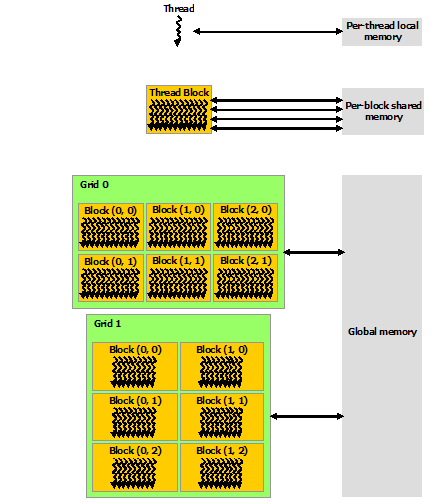
\includegraphics[width=0.4\textwidth]{chap3/memory-hierarchy}}
        \hspace{1cm}
        \subfigure[硬件组织]{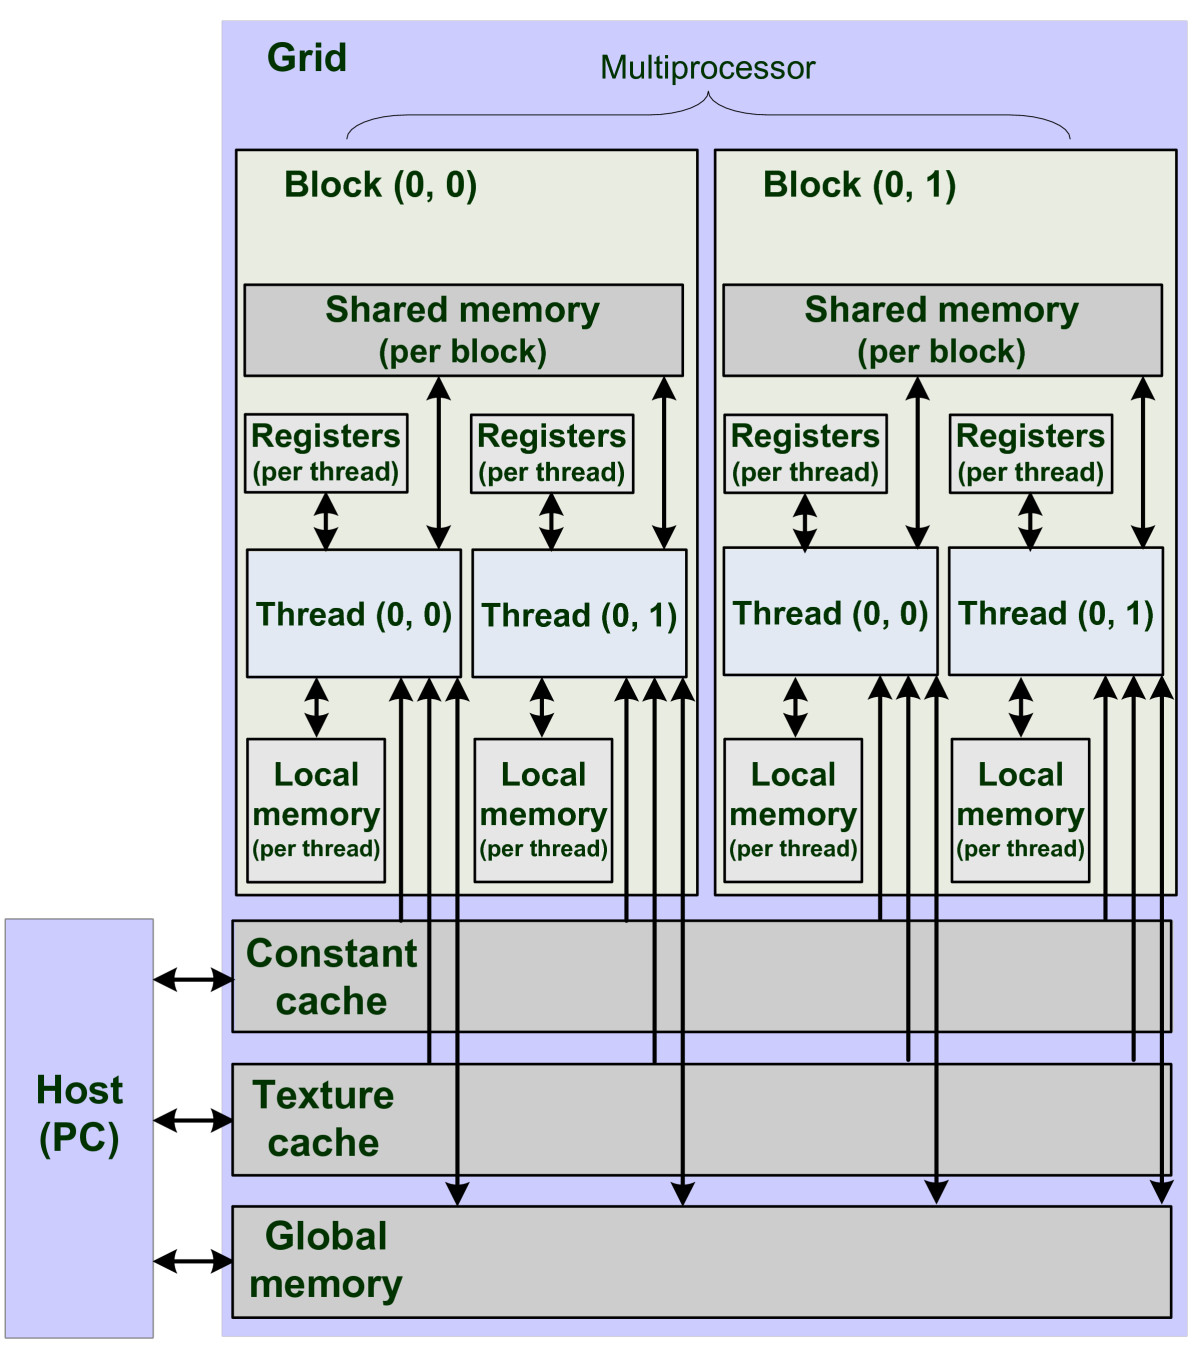
\includegraphics[width=0.4\textwidth]{chap3/memory-model}}
        \caption{内存模型}
      \end{figure}
      并且CUDA还提供了两种所有线程都可以访问的只读内存:常量内存与贴图内存。全局、常量与贴图内存是为了图形渲染流水线特殊优化的内存,与CPU内存相比有一些特殊功能。例如贴图内存提供了不同的访问模式、数据滤镜。
      \par
      实际的硬件当中,每个SM拥有一个所有线程共享的寄存器堆与一个共享内存,这是访问速度最快的内存,平均1Cycle就可以访问到。寄存器是每个进程独有的不会产生冲突,线程的本地内存在寄存器当中,如果线程使用的寄存器过多,则多余的数据会被存放在全局内存当中,造成严重的性能损失。每个SM的共享内存是有限的,并且会产生冲突,如果线程访问共享内存时有冲突,将会影响性能,产生最多1024Cycle的延迟。
      \par
      线程在访问常量内存时会把数据向周围的线程进广播,如果周围的进程也用到了相同的数据,则会大幅减少延迟。贴图内存适合访问在二维上规则的数据,但是在使用前需要先进行绑定。
      \par
      除此之外,每个SM还拥有L1与L2缓存,共享内存与寄存器是L1缓存的一部分,线程访问全局内存时需要经过L1与L2缓存,访问贴图内存是只经过L2缓存\cite{kirk2007nvidia}。
    \subsection{异构计算编程}
      CUDA编程模型假定CUDA线程在分离的硬件设备上作为主机的协处理器来运行C程序,在这种情况下,核函数执行在GPU上,剩余部分由CPU来执行。
      \begin{figure}[htp]
        \centering
        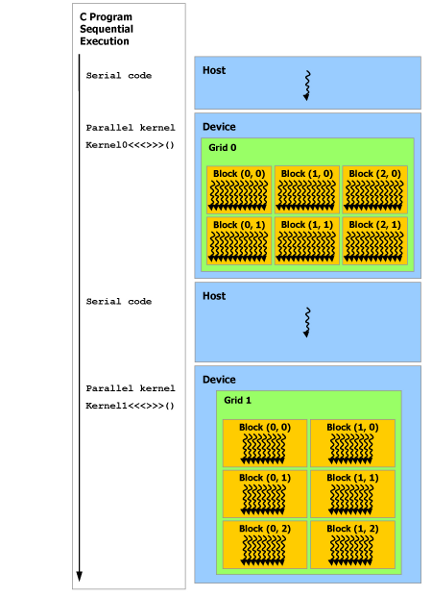
\includegraphics[width=0.5\textwidth]{chap3/heterogeneous-programming}
        \caption{异构计算模型}
      \end{figure}
      \par
      CUDA编程模型同样假定主机与设备同时在DRAM维护独有的内存空间,这两个内存被称为主机内存与设备内存。因此,一个程序需要通过CUDA运行时来管理全局、常量与贴图内存,使它们对核函数可见。也就是说,主机需要分配、释放设备内存,也需要控制只主机与设备内存的数据交换。
    \subsection{计算能力}
      计算能力,或者说SM版本,通常用一个版本数字来表示。由于NVIDIA的显卡架构并不是一成不变的,计算能力表示了显卡的架构以及支持的特性。计算能力由两部分组成,主版本号与副版本号$(x.y)$。主版本号1代表了Tesla架构、2代表了Fermi架构、3代表了Kepler架构、5代表了Maxwell架构。小版本号表示一个架构下的增量改进。
  \section{硬件平台}
    本次实习所使用的GPU是GeForce GTX650,计算能力为3.0,是Kepler架构下的显卡,拥有2个SM,每个SM有192个SP,总共384个SP,单精度浮点运算能力为750GFlops;所用的CPU为Intel E8200@2.66GHz,单精度浮点运算能力为22GFlops。
    \par
    计算能力3.0在每个SM中提供了192个流处理器,4个线程束调度器。并且每个SM拥有一个L1缓存、所有的SM有一个L2缓存。L1缓存用于缓存本地内存(包括寄存器放不下存放在在全局内存中的变量),L2缓存了本地内存与全局内存。在读取内存时,同时向L1与L2缓存进行查询。
    \par
    L1缓存与共享内存由一个硬件来完成,这个硬件提供了64KB的存储大小,并且可以动态的配置L1与共享内存的大小。除此之外,每个SM还提供了一个48KB大小的只读内存用于加速。这两块内存共同构成了L1缓存。
    \par
    CPU方面,Intel E8200提供了SSE4.1指令集,有专门的硬件可以同时运算4个单精度浮点型。在测试中通过gcc的优化开关打开。
  \section{计算精度}
    浮点运算的标准是IEEE 754-2008,在计算能力1.2之后的GPU都支持这一标准下的双精度运算\cite{whitehead2011precision},所有的NVIDIA GPU都支持这一标准下的单精度运算。但是GPU与CPU实现这一标准的方法不同,导致运算结果也会不同,例如,FMA(Fused Multiply-Add)指令可以通过一条指令运算$(X*Y+Z)$的结果,CUDA可以直接支持这条指令。对于x86 CPU来说,由于最初的x87 FPU在计算浮点运算时使用80bit的浮点运算单元,在单个运算上的精度不差于GPU,但是由于多次迭代的原因,在运算$(X*Y+Z)$时,可能会造成精度丢失。除此之外,x87 FPU由于多次进行精度转换,还能能产生不可预测的运算结果,为了让算法的结果具有对比性,编译时将强制CPU使用SSE指令进行浮点运算。